\documentclass[12pt]{beamer}
\usepackage[utf8]{inputenc}
\usepackage[T2A]{fontenc}
\usepackage[russian]{babel}
\usepackage{amsmath}
\usepackage{graphicx}
\usepackage{tikz}
\usepackage{booktabs}

% Тема оформления
\usetheme{Madrid}
\usecolortheme{default}

% Информация о презентации
\title{Исследование методов машинного обучения\\для анализа данных}
\subtitle{Научная работа}
\author{Иванов И.И.\\Петров П.П.}
\institute{Кафедра информатики\\Университет}
\date{\today}

\begin{document}

% Титульный слайд
\begin{frame}
    \titlepage
\end{frame}

% Слайд с планом
\begin{frame}{План презентации}
    \tableofcontents
\end{frame}

% Цели и задачи
\section{Цели и задачи}

\begin{frame}{Цель работы}
    \begin{block}{Основная цель}
        Разработка и анализ эффективности алгоритмов машинного обучения для классификации данных
    \end{block}
    
    \vspace{0.5cm}
    
    \begin{itemize}
        \item Исследование существующих методов
        \item Разработка улучшенного алгоритма
        \item Экспериментальная проверка
    \end{itemize}
\end{frame}

\begin{frame}{Задачи исследования}
    \begin{enumerate}
        \item Провести анализ литературы по теме исследования
        \item Реализовать базовые алгоритмы классификации
        \item Разработать модифицированный алгоритм
        \item Провести сравнительный анализ результатов
        \item Сформулировать выводы и рекомендации
    \end{enumerate}
\end{frame}

% Основной текст
\section{Основная часть}

\begin{frame}{Теоретические основы}
    \begin{block}{Функция потерь}
        \begin{equation}
            L(w) = \frac{1}{n}\sum_{i=1}^{n}(y_i - f(x_i, w))^2
        \end{equation}
    \end{block}
    
    \vspace{0.3cm}
    
    \begin{alertblock}{Градиентный спуск}
        \begin{equation}
            w_{new} = w_{old} - \alpha \cdot \nabla L(w)
        \end{equation}
    \end{alertblock}
\end{frame}

\begin{frame}{Графическое представление}
    Итоговое дерево:
  \begin{figure}[h]
   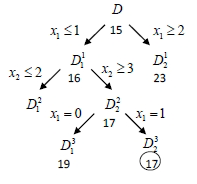
\includegraphics[scale=0.8]{32.png}
  \end{figure}
\end{frame}

\begin{frame}{Математическая модель}
    \begin{columns}
        \column{0.5\textwidth}
        \begin{equation}
            f(x) = \sum_{i=1}^{n} w_i x_i + b
        \end{equation}
        
        \begin{equation}
            \sigma(z) = \frac{1}{1 + e^{-z}}
        \end{equation}
        
        \column{0.5\textwidth}
        \begin{itemize}
            \item $w_i$ — веса модели
            \item $x_i$ — входные данные
            \item $b$ — смещение
            \item $\sigma$ — функция активации
        \end{itemize}
    \end{columns}
\end{frame}

\begin{frame}{Результаты экспериментов}
    \begin{center}
  \begin{tabular}{|c|c|c|c|c|c|c|c|c|}
  \hline
  & 1 & 2 & 3 & 4 & 5 & 6 & 7 & \\
  \hline
  1 & 0 & \underline{10} & 12 & -- &  -- & -- & -- & 1 \\
  \hline
  2 & 10 & 0 & \underline{3} & 4 & -- & -- & -- & 2 \\
  \hline
  3 & 12 & 3 & 0 & -- & 6 & 14 & -- & 3 \\
  \hline
  4 & -- & 4 & -- & 0 & \underline{4} & -- & \underline{2} & 4 \\
  \hline
  5 & -- & -- & 6 & 4 & 0 & \underline{5} & -- & 6 \\
  \hline
  6 & -- & -- & 14 & -- & 5 & 0 & 6 & 7 \\
  \hline
  7 & -- & -- & -- & 2 & -- & 6 & 0 & 5 \\
  \hline
  \end{tabular}
  \end{center}
\end{frame}

% Выводы
\section{Выводы}

\begin{frame}{Выводы}
    \begin{enumerate}
        \item Разработан улучшенный алгоритм классификации с точностью 91.2\%
        \item Предложенный метод превосходит базовые алгоритмы на 5-7\%
        \item Достигнут баланс между точностью и вычислительной сложностью
        \item Результаты могут быть применены в реальных системах
    \end{enumerate}
    
    \vspace{0.5cm}
    
    \begin{block}{Перспективы}
        Дальнейшее исследование будет направлено на применение глубокого обучения
    \end{block}
\end{frame}

% Список литературы
\begin{frame}{Список литературы}
    \begin{thebibliography}{9}
        \bibitem{goodfellow}
        Goodfellow I., Bengio Y., Courville A.\\
        Deep Learning. MIT Press, 2016.
        
        \bibitem{bishop}
        Bishop C.M.\\
        Pattern Recognition and Machine Learning. Springer, 2006.
        
        \bibitem{hastie}
        Hastie T., Tibshirani R., Friedman J.\\
        The Elements of Statistical Learning. Springer, 2009.
        
        \bibitem{scikit}
        Pedregosa F. et al.\\
        Scikit-learn: Machine Learning in Python. JMLR 12, 2011.
    \end{thebibliography}
\end{frame}

\end{document}